\documentclass[article, oneside, oldfontcommands]{abntex2}

\usepackage[alf]{abntex2cite}
\usepackage[T1]{fontenc}
\usepackage[brazil]{babel}
\usepackage{amsmath} % Removido o fullpage para não dar conflito com o geometry
\usepackage{graphicx}
\usepackage{color}
\usepackage[normalem]{ulem}
% \usepackage{fancyhdr} % Comentado para evitar conflito com abntex2
\usepackage[top=3.0cm, left=3cm, bottom=2cm, right=2cm, headheight=75pt]{geometry} 
\usepackage{amssymb}
\usepackage{float}
\usepackage{indentfirst}
\usepackage[utf8]{inputenc}
\usepackage{enumerate}
\usepackage{booktabs} 
\usepackage{siunitx}  
% \usepackage{titlesec} % Comentado para evitar conflito com abntex2
\usepackage{subcaption} % Pacote essencial para subfiguras
\usepackage{hyperref}
\usepackage{cleveref}

% --- Configurações ABNT (Fonte e Espaçamento) ---
\usepackage{helvet} 
\renewcommand{\familydefault}{\sfdefault} 
\OnehalfSpacing % <-- Comando nativo para espaçamento 1.5 no texto
% ------------------------------------------------

\newcommand{\uvec}[1]{\boldsymbol{\hat{\textit{#1}}}}
\setlength{\parindent}{1.25cm} 

\graphicspath{{image/}}

\begin{document}

% --- INÍCIO DA CAPA ---
\thispagestyle{empty} % Remove o número da página apenas desta folha
\begingroup % Inicia um grupo para o espaçamento não vazar pro resto do texto

% Cabeçalho da Capa (Texto à esquerda e Logo à direita alinhados por baixo)
\noindent
\begin{minipage}[b]{0.7\textwidth}
    \small
    \textbf{Matéria:} TÓPICOS - ENGENHARIA DE CIRCUITOS IMPRESSOS\\[0.1cm]
    \textbf{Professor:} SEBASTIEN ROLAND MARIE JOSEPH RONDINEAU
\end{minipage}%
\begin{minipage}[b]{0.3\textwidth}
    \raggedleft
    
\includegraphics[width=2.5cm]{unb_logo.png}
\end{minipage}

\vspace{0.15cm} 
\noindent\rule{\textwidth}{0.4pt} 

\vfill 

\begin{center}
    {\huge \textbf{Quadrature Hybrid Coupler Circular}}\\[0.5cm]
    {\Large Trabalho Final da Disciplina}
\end{center}

\vfill 

\begin{center}
    {Gustavo Emmanuel dos Santos Rodrigues} - 232036878 \\
    {Arthur Vilas Boas Laterza} - 232037374 \\
    \vspace{0.5cm}
    \today
\end{center}

\endgroup
% --- FIM DA CAPA ---

\newpage
\pagenumbering{arabic}
\setcounter{page}{1}
\pagestyle{plain}

% -----------------------------------------

\section{Resumo}

Este documento trata de uma apresentação de um trabalho final para a disciplina de Engenharia de Circuitos Impressos, focado no desenvolvimento e análise de um \textit{Quadrature Hybrid Coupler}, projetado em formato circular e a uma frequência de 2.4 GHz. O trabalho abrange a concepção, simulação e avaliação do desempenho do dispositivo, destacando suas aplicações práticas e relevância no campo da engenharia. 


\section{Objetivos}

Tem-se como objetivo aprender com a prática o conteúdo previsto na ementa da disciplina, desenvolvendo uma placa de circuito impresso que implementa a funcionalidade proposta, um componente aplicável em sistemas de micro-ondas e comunicações. Também se busca aprimorar habilidades em simulação, análise de desempenho e compreensão dos princípios de funcionamento de circuitos impressos, contribuindo para a formação técnica e profissional dos integrantes.

\section{Introdução}

O acoplador híbrido em quadratura consolida-se como um componente fundamental em circuitos de micro-ondas. Este dispositivo passivo de quatro portas tem como função principal dividir ou combinar sinais de potência, garantindo uma defasagem exata de 90 graus entre as suas portas de saída. Devido à sua capacidade de fornecer alta isolação e acoplamento eficiente com perdas mínimas, ele é amplamente empregado em blocos críticos de sistemas modernos, incluindo redes de alimentação de antenas, moduladores I/Q, misturadores balanceados e sistemas de radar.

Estruturalmente, o acoplador em quadratura é composto por quatro braços de linhas de transmissão com comprimentos de um quarto de onda ($\lambda/4$), frequentemente fabricados utilizando tecnologias planas, como microstrip ou stripline. Em sua topologia retangular clássica (como ilustrado na Figura \ref{fig:sub_retangular}), o sinal injetado na porta de entrada é dividido equitativamente (3 dB) entre a porta direta e a porta acoplada, enquanto a quarta porta permanece isolada. No entanto, este projeto propõe o desenvolvimento e a análise de uma versão deste modelo implementada no modo circular (Figura \ref{fig:sub_circular}).

\begin{figure}[H]
    \centering
    % Primeira subfigura (a)
    \begin{subfigure}[b]{0.65\textwidth}
        \centering
        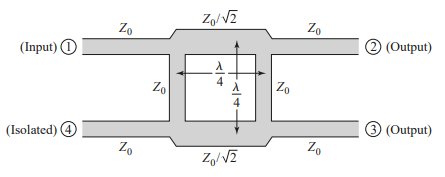
\includegraphics[width=\linewidth]{quadrada.png}
        \caption{Topologia retangular clássica}
        \label{fig:sub_retangular}
    \end{subfigure}\hfill
    % Segunda subfigura (b)
    \begin{subfigure}[b]{0.5\textwidth}
        \centering
        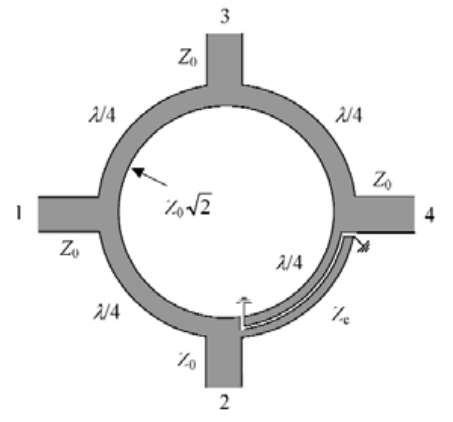
\includegraphics[width=0.8\linewidth]{referencia.png} % Ajustei para 0.8 para ficar mais legível, mas pode voltar para 0.45 se preferir
        \caption{Topologia circular proposta}
        \label{fig:sub_circular}
    \end{subfigure}
    
    \caption{Comparativo das topologias do Quadrature Hybrid Coupler}
    \label{fig:calculadora1}
\end{figure}

Diferentemente da topologia convencional de ramos retos, a implementação do híbrido em quadratura na geometria circular visa mitigar as descontinuidades eletromagnéticas inerentes às quinas de 90 graus. Em circuitos de alta frequência, tais ângulos retos introduzem indutâncias e capacitâncias parasitas significativas que podem degradar a largura de banda, alterar a frequência de ressonância e comprometer a isolação entre as portas. A adoção de uma estrutura circular promove uma transição de impedância geométrica mais suave e contínua, otimizando a distribuição das linhas de campo elétrico e magnético ao longo dos ramos de acoplamento. \\

\noindent \cite{pozar2011microwave} \cite{sinchangreed2011design} \cite{stec2018quadrature} \cite{rahman2018quadrature} \cite{zeng2022compact} \cite{grebennikov2008power}

\section{Metodologia}

A metodologia adotada para o desenvolvimento deste projeto divide-se em quatro etapas sequenciais: fundamentação teórica, projeto e simulação eletromagnética, prototipagem da placa de circuito impresso (PCB) e, por fim, a validação experimental no laboratório.

Inicialmente, será realizado um estudo aprofundado para a compreensão teórica dos fenômenos de alta frequência abordados na ementa. 
Esta etapa contemplará a análise matemática do \textit{Quadrature Hybrid Coupler} em sua topologia circular, aplicando-se a Análise de Modos Par e Ímpar (\textit{Even-Odd Mode Analysis}) para o equacionamento analítico do dispositivo. Esse estudo culminará no desenvolvimento da Matriz de Espalhamento ($[S]$), que servirá como modelo ideal para a caracterização do funcionamento do circuito.

Para a fase de dimensionamento físico e sintonia, serão utilizadas as ferramentas de simulação do \textit{software Keysight Advanced Design System (ADS)}. O procedimento iniciará com simulações no nível esquemático utilizando modelos ideais de linhas de transmissão, evoluindo progressivamente para a modelagem em tecnologia de microfita. 
Nesta transição, serão inseridas as propriedades físicas reais do substrato a ser utilizado na fabricação (como constante dielétrica $\varepsilon_r$, tangente de perdas $\tan \delta$ e espessura da placa). 

Com o \textit{layout} gerado, será executada a simulação eletromagnética (EM) no ADS para computar os efeitos parasitas e as descontinuidades geométricas das trilhas e curvas. O foco desta etapa será a otimização paramétrica para garantir que os indicadores de desempenho, como o casamento de impedância ($S_{11}$), o acoplamento com divisão de potência equitativa ($S_{21}$ e $S_{31}$), a isolação entre portas ($S_{41}$) e o desfasamento exato de 90 graus, atendam às especificações dentro da largura de banda de operação desejada.

Por fim, o \textit{layout} otimizado será encaminhado para a fabricação. A validação do projeto ocorrerá por meio da caracterização experimental do protótipo físico utilizando um Analisador de Rede Vetorial (VNA). Os parâmetros S medidos na bancada serão confrontados diretamente com os dados extraídos das simulações computacionais e com os limites estabelecidos pela literatura teórica, permitindo uma análise crítica das métricas alcançadas e das eventuais não idealidades inerentes ao processo de fabricação. 

\section{Cronograma}

A Tabela \ref{tab:cronograma} apresenta as etapas do projeto distribuídas ao longo das doze semanas estipuladas para a conclusão do trabalho final.

\begin{table}[H]
    \centering
    \caption{Cronograma de atividades do projeto (12 semanas)}
    \label{tab:cronograma}
    \vspace{0.3cm}
    \renewcommand{\arraystretch}{1.3}
    \resizebox{\textwidth}{!}{%
    \begin{tabular}{l c c c c c c c c c c c c}
        \toprule
        \textbf{Atividades} & \textbf{S1} & \textbf{S2} & \textbf{S3} & \textbf{S4} & \textbf{S5} & \textbf{S6} & \textbf{S7} & \textbf{S8} & \textbf{S9} & \textbf{S10} & \textbf{S11} & \textbf{S12} \\
        \midrule
        Revisão Bibliográfica teórica           & $\bullet$ & $\bullet$  &   &   &   &   &   &   &   &   &   &   \\
        Cálculo analítico dos parâmetros        &   &   & $\bullet$ & $\bullet$ &   &   &   &   &   &   &   &   \\
        Design no software ADS                  &   &   &   &   & $\bullet$ & $\bullet$ & $\bullet$ &   &   &   &   &   \\
        Simulação eletromagnética               &   &   &   &   &   &   & $\bullet$ & $\bullet$ &    &   &   &   \\
        Otimização e ajustes no layout (ADS)          &   &   &   &   &   &   &   & $\bullet$ & $\bullet$ &  &   &   \\
        Design no software HFSS                 &   &   &   &   &   &   &   &   & X & X &   &   \\
        Simulação eletromagnética               &   &   &   &   &   &   &   &   &   & X & X &    \\
        Análise de dados e escrita do relatório &   &   &   &   &   & X & X & X & X & X & X & X \\
        \bottomrule
    \end{tabular}%
    }
\end{table}

\section{Resultados esperados}

Para um Acoplador Híbrido de Quadratura (que geralmente tem 4 portas), os resultados esperados giram em torno do comportamento ideal dos Parâmetros S (Espalhamento) na frequência central de operação do projeto. É esperado que seja concluído os tópicos:

\begin{itemize}
    \item \textbf{Divisão de Potência (Insertion Loss)}: Espera-se que o sinal de entrada (Porta 1) seja dividido igualmente entre as portas de saída (Portas 2 e 3). Portanto, os parâmetros de transmissão idealmente devem estar próximos de -3 dB na frequência de projeto.
    \item \textbf{Diferença de Fase (Quadratura)}: O principal atrativo deste dispositivo é a defasagem. Espera-se observar uma diferença de fase de exatamente 90 graus ($\pi/2$) entre os sinais que chegam às duas portas de saída.
    \item \textbf{Casamento de Impedância (Return Loss)}: Espera-se que haja o mínimo de reflexão possível na porta de entrada, o que significa que o coeficiente de reflexão deve ser bastante atenuado (idealmente muito menor que -10 dB ou tendendo a zero na escala linear) na frequência central.
    \item \textbf{Isolamento}: A quarta porta (Porta isolada) não deve receber potência idealmente. O resultado esperado é um alto isolamento (um valor muito baixo em dB) entre a porta de entrada e a porta isolada.
\end{itemize}

\section{Desenvolvimento}

O desenvolvimento prático do trabalho foi dividido nas seguintes seções:
\begin{itemize}
    \item \textbf{\boldmath ADS:}
    \begin{itemize}
        \item Design de modelo de linhas de transmissão ideais.
        \item Design de modelo de linhas de transmissão com perdas (microstrip).
        \item Geração do Layout e simulação EM.
        \item Otimização EM com parâmetros de varredura (Parameters Sweep).
    \end{itemize}
    \item \textbf{\boldmath HFSS:}
    \begin{itemize}
        \item Design do modelo.
    \end{itemize}
\end{itemize}

\subsection{Design no software ADS}

\subsubsection{Design de modelo de linhas de transmissão ideais}

O primeiro passo no desenvolvimento do acoplador é a criação do modelo ideal para a visualização dos valores de parâmetros S alvo. Para isso basta criar um esquemático e, com a utilização da biblioteca "TLines-Ideal", projetar o modelo do circuito visto na \cref{fig:sub_retangular}. No modelo ideal pode ser montado com o formato do acoplador quadrado, pois como estamos trabalhando com o modelo ideal isto se torna irrelevante. Logo, o esquemático criado é mostrado na \cref{fig:esquematico_ideal}.

\begin{figure}[H]
\begin{center}
    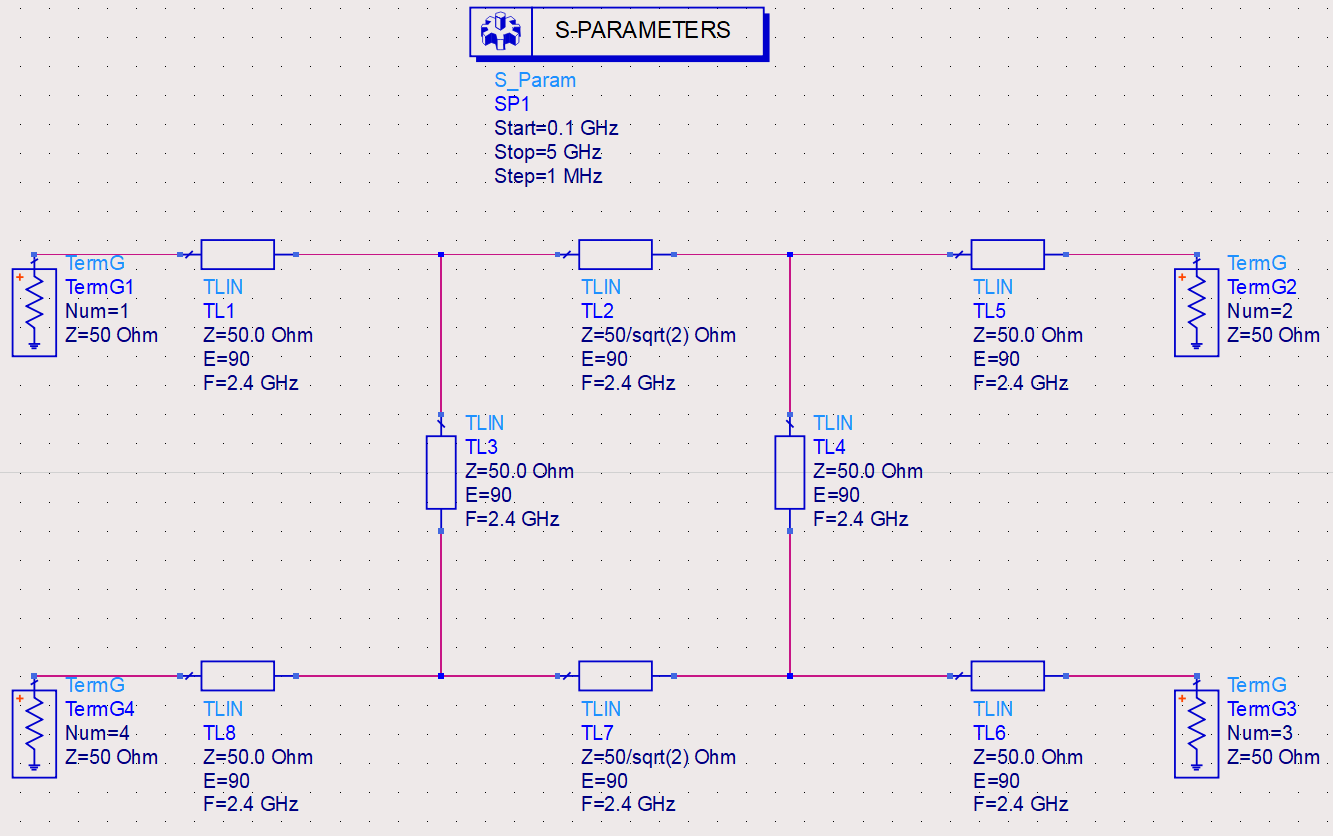
\includegraphics[width=0.7\textwidth]{esquematico_ideal}
\end{center}
\caption{Esquemático do modelo de linhas de transmissão ideais do acoplador em quadratura.}\label{fig:esquematico_ideal}
\end{figure}

Por meio do esquemático criado, foi possível gerar os gráficos de parâmetros S por meio da ferramenta "Simulate", como visto na \cref{fig:grafico_ideal}. 

\begin{figure}[H]
\begin{center}
    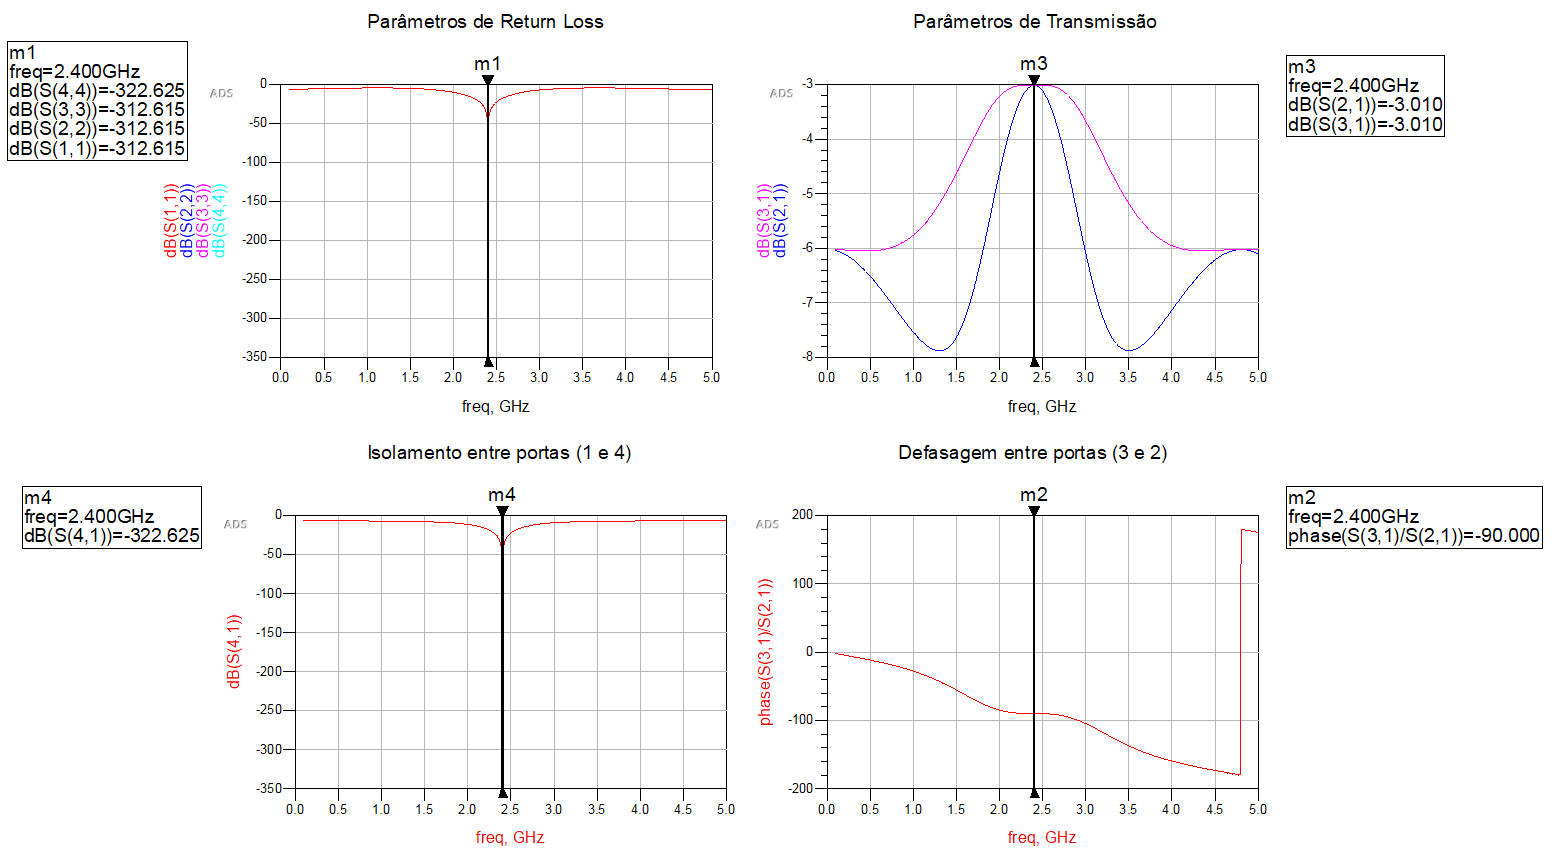
\includegraphics[width=1\textwidth]{grafico_ideal}
\end{center}
\caption{Parâmetros S do modelo de linhas de transmissão ideais.}\label{fig:grafico_ideal}
\end{figure}

Com os resultados obtidos foi possível observar que, conforme previa a teoria, teriamos um divisão perfeitamente igual de potência para as portas 2 e 3 (considerando a porta 1 como entrada) com defasagem de 90°. Além disso, podemos notar que os casamento de cada porta é perfeito ($\Gamma = 0$) e existe um isolamento total da porta 4 com relação à porta 1.

\subsubsection{Design de modelo de linhas de transmissão com perdas (microstrip)}

A próxima etapa consiste no projeto do esquemático utilizando linhas de transmissão com perdas, sendo elas perdas ôhmicas e dielétricas. Logo, foi necessário escolher um substrato que atendesse as demandas de custo-benefício e desempenho. 

O substrato escolhido foi o modelo RO4003C da \textit{Rogers Corporation}, o qual provê uma constante dielétrica extremamente controlada, fazendo com que varie pouco. Isso é benéfico para o projeto pois o acoplador híbrido depende em um comprimento de quarto de onda ($\lambda/4$) preciso para atingir os valores esperados. Além disso, este substrato também contribui para a diminuição das perdas dielétricas, com uma baixa tangente de perdas. 

\begin{table}[H]
    \centering
    \caption{Substrato RO4003C}
    \label{tab:substrato}
    \vspace{0.3cm}    % Espaço entre o título e a tabela
    \renewcommand{\arraystretch}{1.5} % Aumenta o espaçamento das linhas
    \begin{tabular}{|l|c|}    % Define o alinhamento das colunas (l, c, r) e adiciona uma linha vertical entre elas
    \hline    % cria linha horizontal
    Constante Dielétrica relativa & $\varepsilon = 3,55$ \\
    \hline    % cria linha horizontal
    Tangente de Perdas Dielétricas & $tan \delta = 0,0021$ \\
    \hline    % cria linha horizontal
    Substrate thickness & $0.508 mm$ \\
    \hline
    Conductor thickness & $0.035 mm$ \\
    \hline
    % ...
    \end{tabular}
 
    \vspace{0.4cm} 
\end{table}

Para a montagem utilizamos os componentes da biblioteca "TLines-Microstrip", que contemplam vários tipos de linhas de transmissão, com diversos formatos. Para criarmos o modelo do acoplador circular foi necessário utilizar os componentes de curvas circulares. O esquemático projetado é mostrado na \cref{fig:esquematico_com_perdas}.

\begin{figure}[H]
\begin{center}
    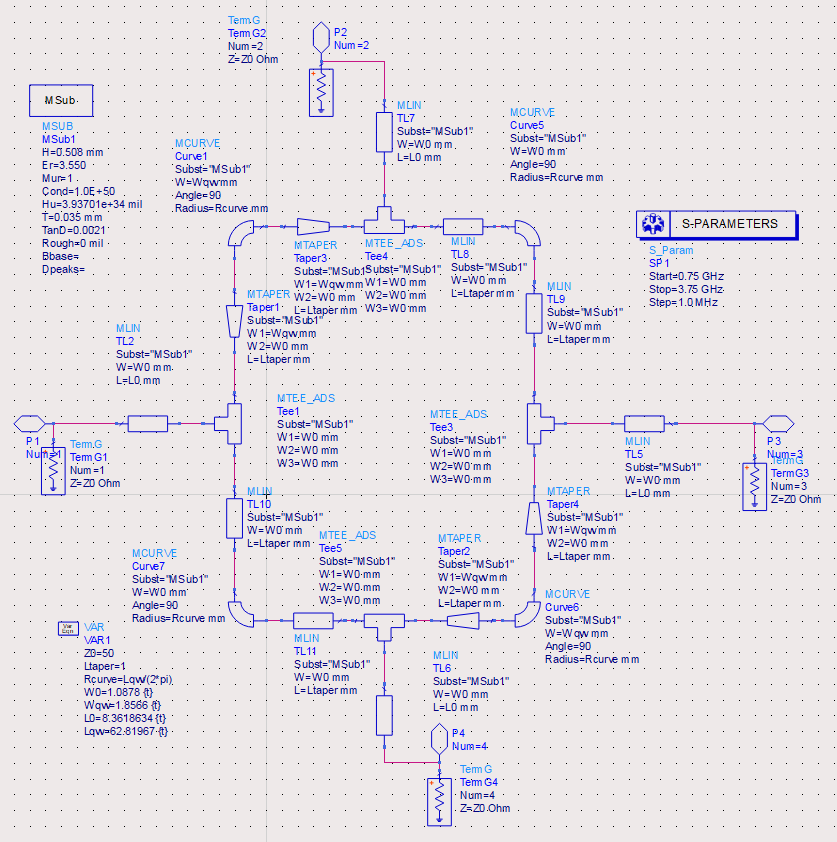
\includegraphics[width=0.7\textwidth]{esquematico_com_perdas}
\end{center}
\caption{Esquemático do acoplador utilizando componentes com perdas.}\label{fig:esquematico_com_perdas}
\end{figure}

Para a criação deste esquemático foi visto necessário o uso da ferramenta do "LineCalc" para a obtenção das dimensões de cada trecho da trilha (comprimento L e largura W), considerando os valores referentes de impedância e comprimento de onda das mesmas. Como visto na \cref{fig:linecalc}.

\begin{figure}[H]
\begin{center}
    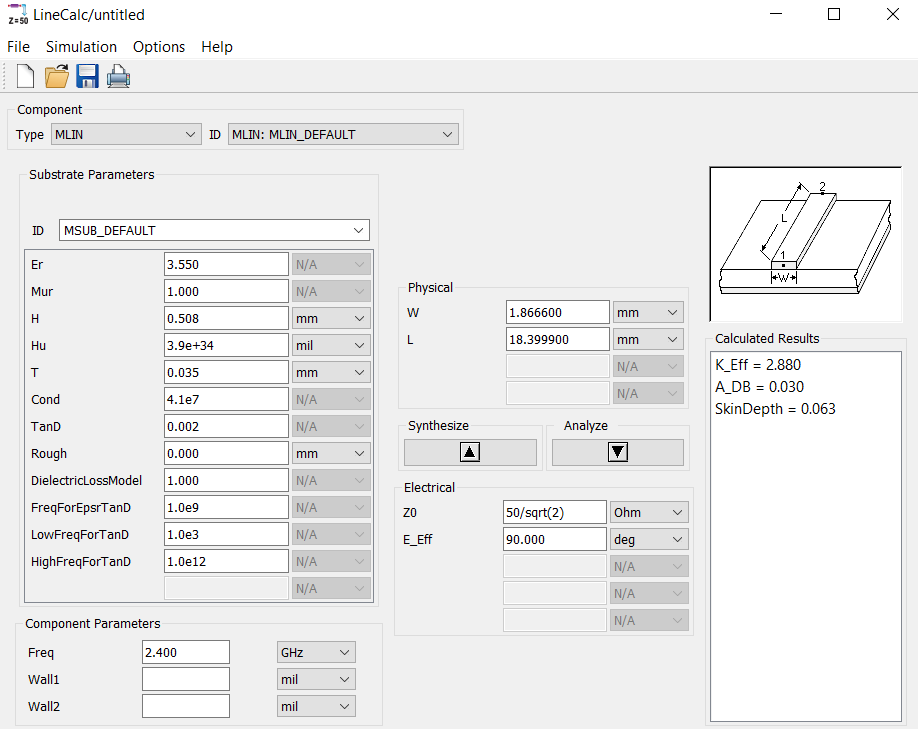
\includegraphics[width=0.7\textwidth]{linecalc}
\end{center}
\caption{Ferramenta do LineCalc.}\label{fig:linecalc}
\end{figure}

Depois foi feito uma simulação de 0.75GHz até 3.75GHz com passos de 1MHz, o que possibilitou que pudéssemos visualizar a frequência desejada no centro do gráfico. Como esperado os valores para os parâmetros S não foram bons de início, logo foi necessário realizar a otimização utilizando a ferramenta "Tuning", que possibilita mudar os valores das variáveis selecionadas manualmente, observando o seu impacto nos valores dos parâmetros S. Foi selecionado as variáveis "Ltaper" (comprimento dos tapers), "W0" (espessura das trilhas conectadas às portas), "L0" (comprimento das trilhas conectadas às portas), Wqw (espessura das trilhas com impedância $Z_{qw}$) e Lqw (comprimento $\lambda/4$), como visto na \cref{fig:tuning}.

\begin{figure}[H]
\begin{center}
    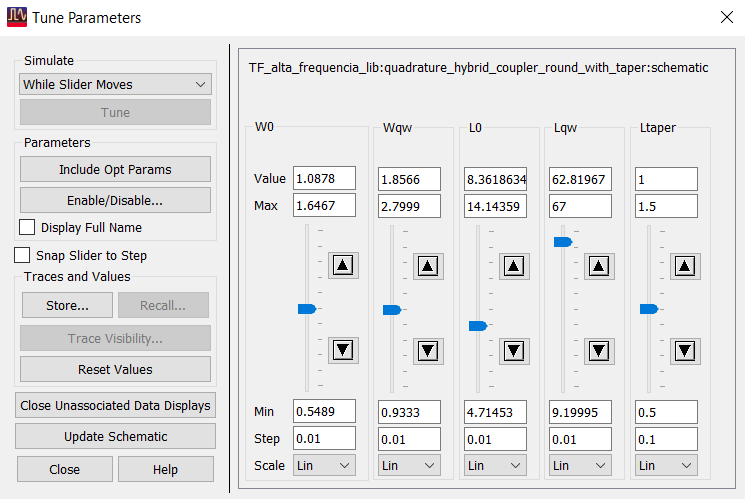
\includegraphics[width=0.7\textwidth]{tuning}
\end{center}
\caption{Ferramenta de otimização "Tuning"}\label{fig:tuning}
\end{figure}

Com os valores das variáveis otimizados, foram obtidos valores mais próximos ao modelo ideal para os parâmetros S. Na \cref{fig:grafico_com_perdas_with_taper}, é possível observar que, similarmente ao modelo ideal, cada porta tem um coeficiente de reflexão (Return Loss) excelente, atingindo $\approx -50 dB$. Adicionalmente, podemos observar também uma divisão de potência muito próxima entre os parâmetros de transmissão ($S_{31}$ e $S_{21}$), além de uma diferença de fase entre as portas 2 e 3 de $\approx 90$°. Por último, nota-se um ótimo valor de bloqueio da transmissão para a porta isolada ($S_{41} \approx -42dB$).

\begin{figure}[H]
\begin{center}
    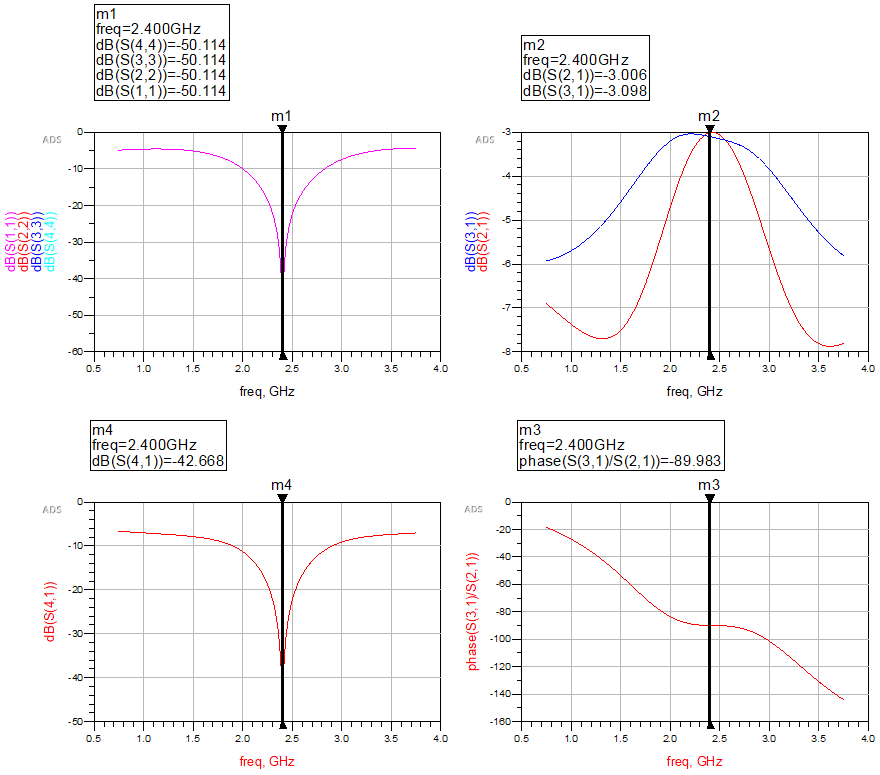
\includegraphics[width=1\textwidth]{grafico_com_perdas_with_taper}
\end{center}
\caption{Parâmetros S do modelo de linhas de transmissão com perdas. }\label{fig:grafico_com_perdas_with_taper}
\end{figure}



\subsubsection{Geração do Layout e simulação EM}

Realizado o esquemático, podemos gerar um layout utilizando a ferramenta "Generate/Update Layout" a partir dele, que representa o arranjo físico do circuito, como mostrado na \cref{fig:layout_with_taper}.

\begin{figure}[H]
\begin{center}
    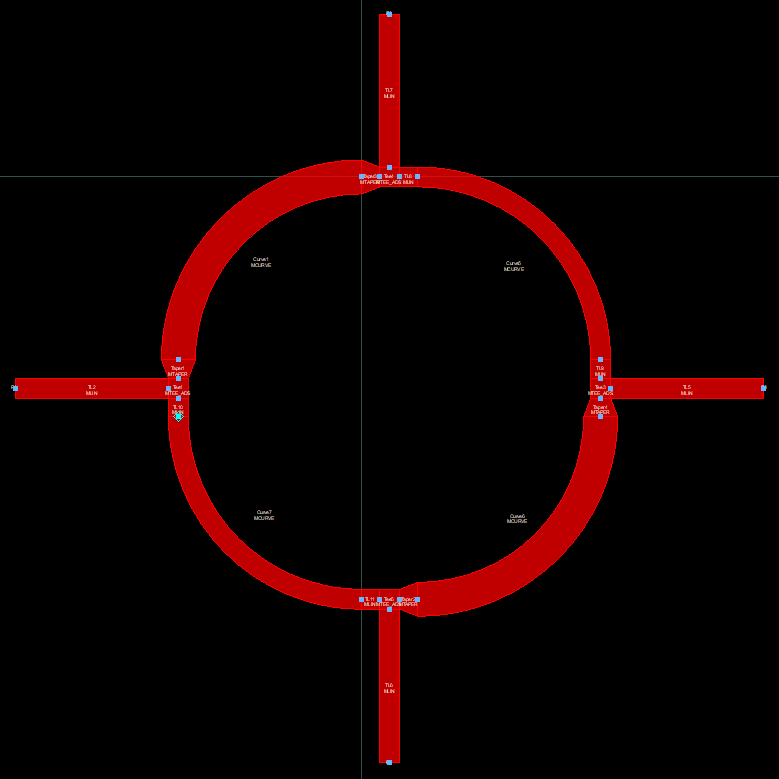
\includegraphics[width=0.6\textwidth]{layout_with_taper}
\end{center}
\caption{Layout do acoplador circular.}\label{fig:layout_with_taper}
\end{figure}

Nota-se o uso do elemento "MTAPER", o qual foi utilizado para suavizar transições abruptas entre impedâncias, como de $Z_0$ para $Z_{QW}$, atenuando os efeitos de bordas nas quinas que, consequentemente, acaba reduzindo o coeficiente de reflexão em cada transição, como visto em \cref{fig:taper}.

\begin{figure}[H]
\begin{center}
    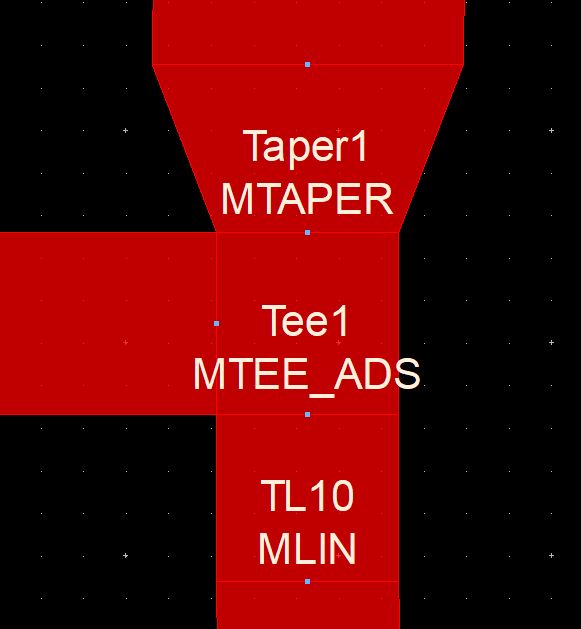
\includegraphics[width=0.4\textwidth]{taper}
\end{center}
\caption{Componente Taper pare diminuir os efeitos de borda.}\label{fig:taper}
\end{figure}

Com o layout gerado, o próximo passo é configurar o dielétrico utilizando a ferramenta "Substrate Editor". De acordo com a \cref{tab:substrato}, podemos preencher os parâmetros do substrato conforme foi feito no esquemático anteriormente.

\begin{figure}[H]
\begin{center}
    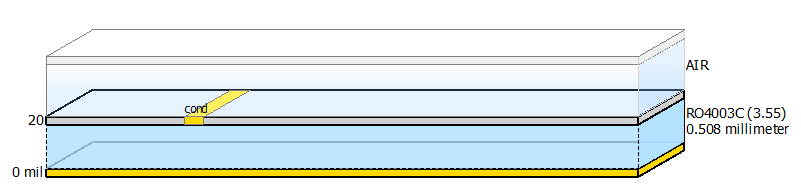
\includegraphics[width=0.7\textwidth]{substrato_configuracao}
\end{center}
\caption{Configuração do substrato no Layout.}\label{fig:substrato_configuracao}
\end{figure}

Configurado o substrato, podemos partir para as configurações da simulação EM. Nessa seção, pode ser adicionado o intervalo de simulação e referenciar o substrato criado. Finalizado o setup, podemos então realizar a simulação do modelo com perdas, agora considerando os efeitos eletromagnéticos.

\begin{figure}[H]
\begin{center}
    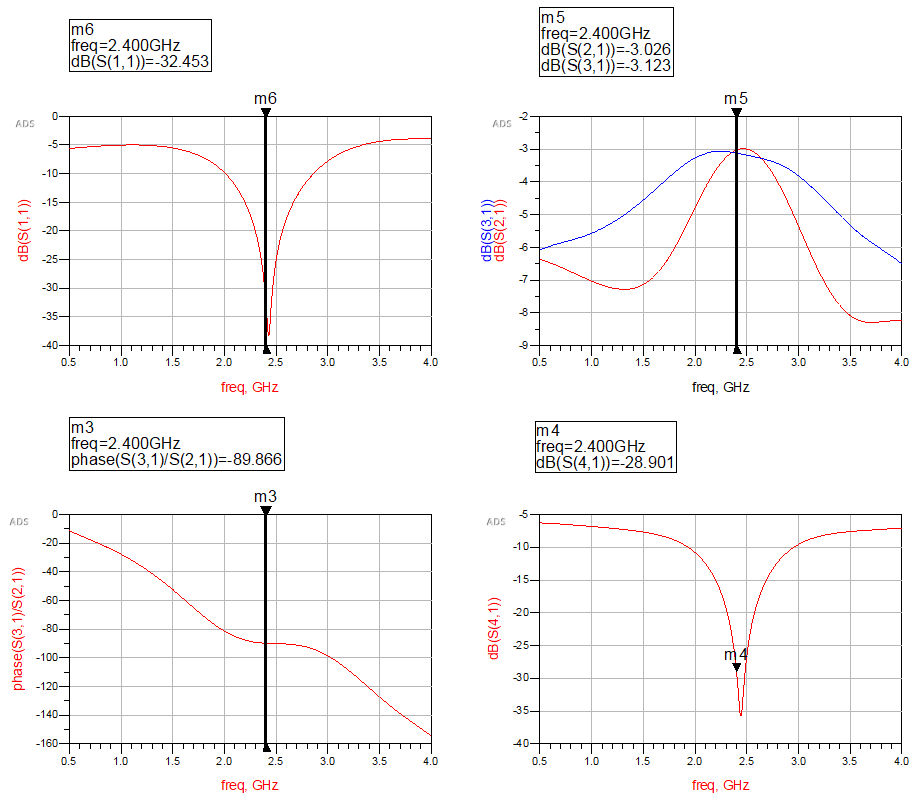
\includegraphics[width=1\textwidth]{grafico_EM_with_taper_ruim}
\end{center}
\caption{Parâmetros S do modelo de linhas de transmissão com perdas eletromagnéticas.}\label{fig:grafico_EM_with_taper_ruim}
\end{figure}

Analisando \cref{fig:grafico_EM_with_taper_ruim}, é possível observar que os resultados, embora satisfatórios, apresentam algumas diferenças quando comparados com o esquemático, já que agora são consideradas condições reais do circuito. Os valores mais satisfatórios são encontados em frequências diferentes da de interesse, por conta das perdas causadas pelos efeitos EM. 

\subsubsection{Otimização EM com parâmetros de varredura (Parameters Sweep)}

Mesmo com valores bons, ainda é possível realizar uma otimização para evoluir os parâmetros S utilizando parâmetros de varredura. Para utilizar o parâmetros de varredura, é necessário criar um symbol do layout criado.

Para fazer isto, o primeiro passo foi criar novos parâmetros no layout com os mesmos valores das variáveis do esquemático, e depois colocar estes parâmetros em cada trecho de trilha do nosso design. Isto é necessário para quando for criado o symbol, ele atribuir estes parâmetros editáveis em suas dimensões. 

Com o symbol criado, basta que dupliquemos nosso esquemático original e, na cópia, substituírmos todos os componentes por este symbol, importando ele no esquemático. Colocamos as portas conectadas diretamente no symbol e depois adicionamos o "Parameters Sweep", através da biblioteca "Simulation-S\_Param".
O resultado desta montagem é exibida na \cref{fig:esquematico_EM_with_taper}.

\begin{figure}[H]
\begin{center}
    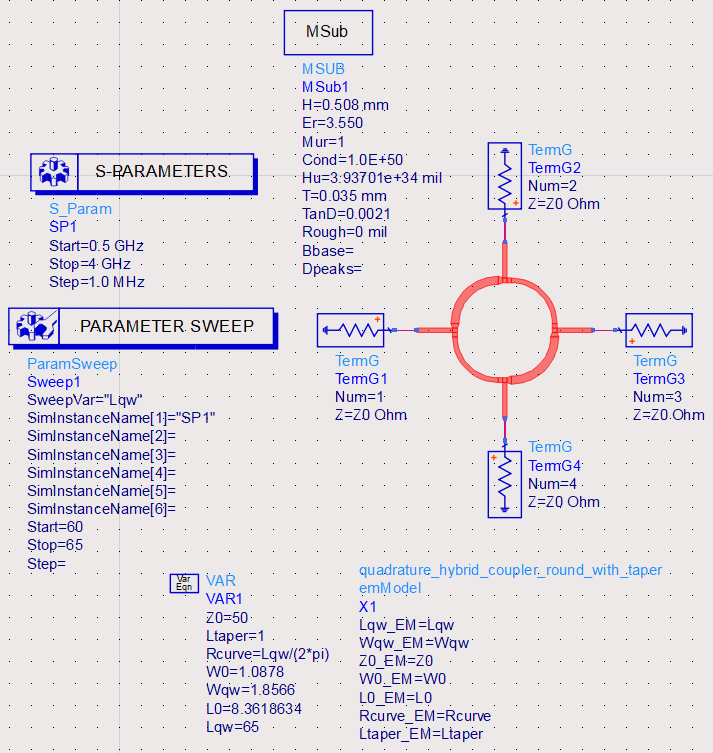
\includegraphics[width=0.7\textwidth]{esquematico_EM_with_taper}
\end{center}
\caption{Esquemático utilizando o symbol extraído do layout.}\label{fig:esquematico_EM_with_taper}
\end{figure}

Para a otimização através de parâmetros de varredura, foi necessário fazer uma série de varreduras com diversas variáveis. Para começar, foi realizada a varredura utilizando a variável Wqw (largura das trilhas de impedâcia $Z_0/\sqrt(2)$) até conseguir os melhores parâmetros S. Logo em seguida, utilizamos a varredura para a variável Lqw (comprimento das trilhas com impedância $Z_0/\sqrt(2)$) para dar um ajuste fino final, como visto na \cref{fig:grafico_sweep_EM_with_taper1}.

\begin{figure}[H]
\begin{center}
    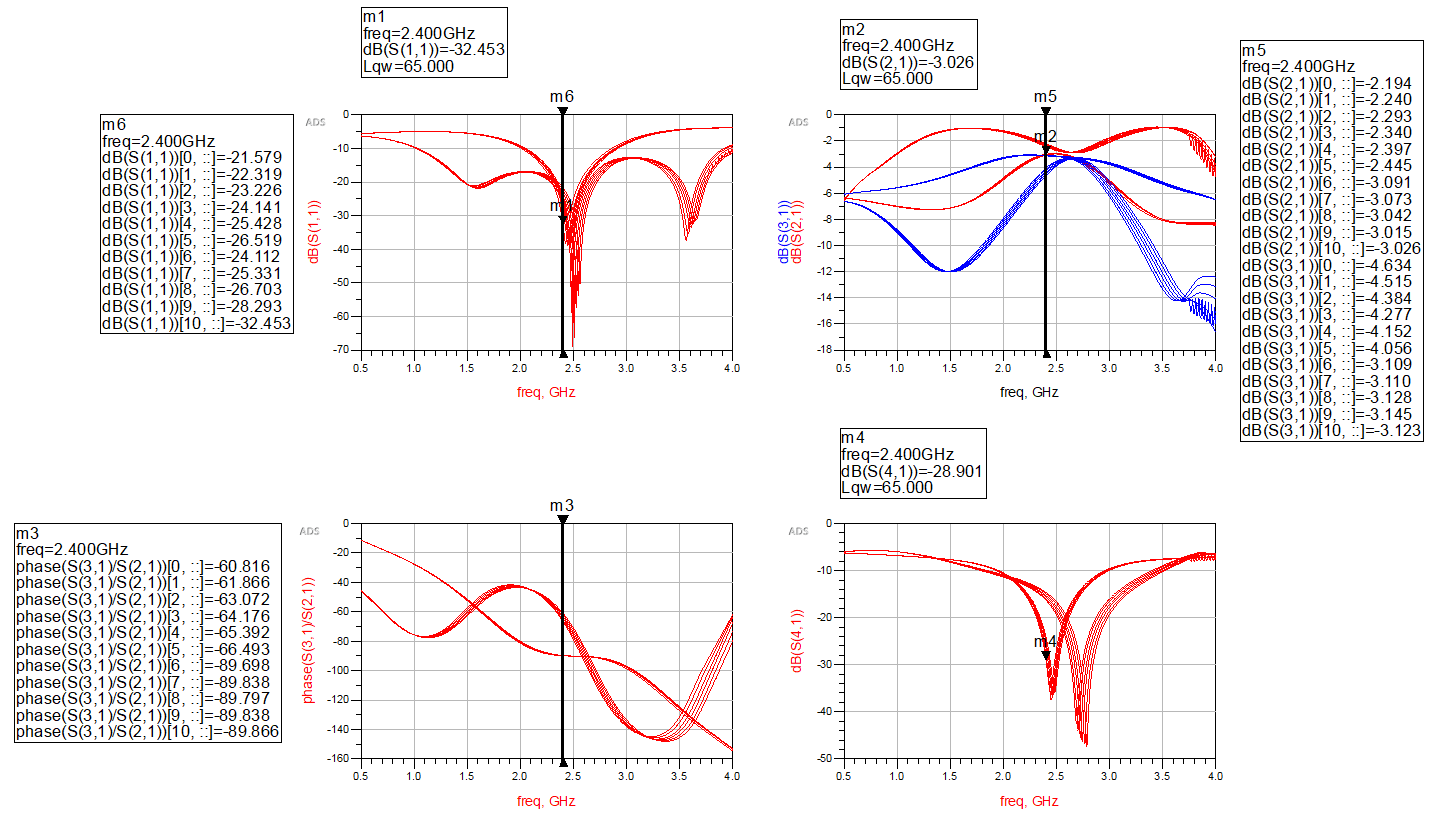
\includegraphics[width=1\textwidth]{grafico_sweep_EM_with_taper1}
\end{center}
\caption{Varredura dos parâmetros de Lqw.}\label{fig:grafico_sweep_EM_with_taper1}
\end{figure}

Ao realizar várias simulações de varredura com diversos valores, foi possível chegar em duas possibilidades interessantes. Nós poderíamos optar por um valor de $S_{11}$ muito baixo, mas como consequência, teríamos uma discrepância maior entre os parâmetros $S_{21}$ e $S_{31}$, ou seja, o sinal seria dividido de forma desigual.
A outra possibilidade seria deixar a divisão de potência o mais precisa possível ($S_{21} \approx S_{31} \approx -3dB$), mantendo um valor de Return Loss baixo para as portas de entrada.

\begin{figure}[H]
\begin{center}
    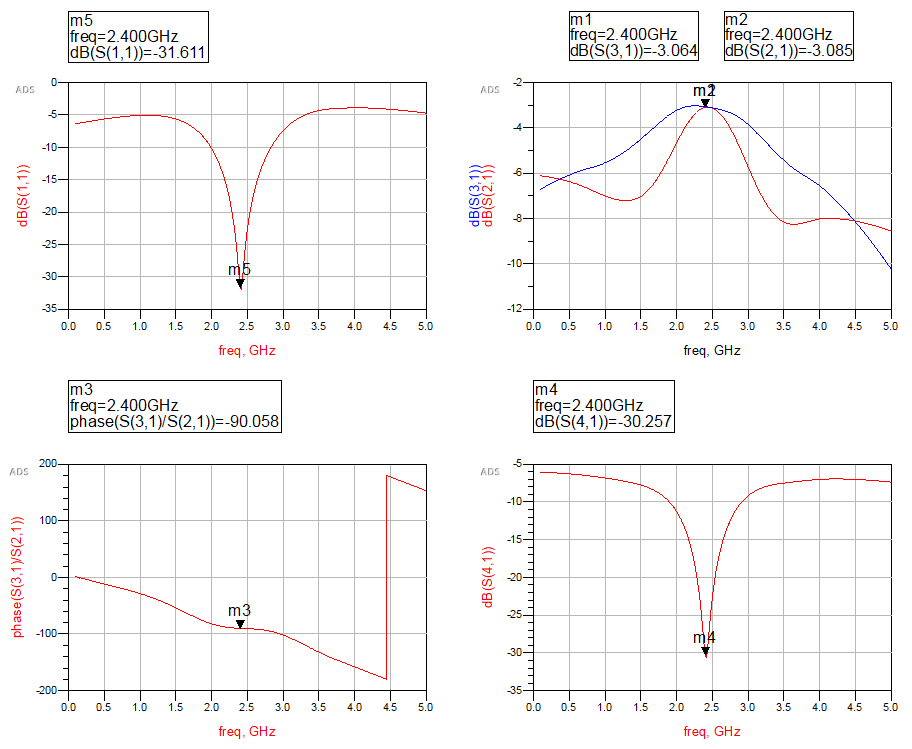
\includegraphics[width=0.7\textwidth]{grafico_EM_with_taper}
\end{center}
\caption{Parâmetros S do modelo de linhas de transmissão com perdas eletromagnéticas após a otimização utilizando parâmetros de varredura.}\label{fig:grafico_EM_with_taper}
\end{figure}

Com muita análise e otimização, chegou-se a conclusão que seria melhor manter valores de $S_{21}$ e $S_{31}$ menos distíntos possível ($S_{21} \approx S_{31} \approx -3dB$), mas tendo em vista também um valor de $S_{11} \lessapprox -30dB$ (reflexão $\Gamma \approx 0$). Esta foi a decisão tomada pois, quando se tinha um valor muito menor para $S_{11}$, os valores de $S_{21}$ e $S_{31}$ começavam a se distanciar bastante, e faria com que uma porta de saída recebesse mais potência do que a outra, o que não é esperado. O resultado desta análise resultou no gráfico mostrado na \cref{fig:grafico_EM_with_taper}


\subsection{Design no software Ansys HFSS}


\section{Conclusão}

Neste laboratório, foi possível realizar com excelência, um bom design para o acoplador híbrido circular de 2,4GHz. Conseguimos extrair ótimos valores para os parâmetros S, tanto para as perdas de retorno, para transferência e divisão de potência com a devida defasagem, e por último, um isolamento perfeito da porta restante. 

Este projeto teve uma função muito importante para a compreensão e entendimento do funcionamento de placas de circuito impresso em altas frequências, onde são necessários os devidos cuidados quanto as perdas ôhmicas e dielétricas. 



\newpage
\bibliography{referencias}

\end{document}